\documentclass{article}

\usepackage{graphicx}
\usepackage{amsmath,amssymb}
\usepackage{gensymb}
\usepackage{mathtools}
\usepackage{etoolbox}
\usepackage{booktabs}
\usepackage{float}
\usepackage{graphicx}
\usepackage{geometry}
\usepackage{multicol}
\usepackage{caption}

\newcommand\mgin{0.5in}
\geometry{
	left=\mgin,
	right=\mgin,
	bottom=\mgin,
	top=\mgin
}

% Set path to import figures from
\graphicspath{{../figures/}}

% Place converted graphics in current directory
\usepackage[outdir=./]{epstopdf}

% Define multicolumn figure-like environment
% from http://tex.stackexchange.com/questions/12262/multicol-and-figures
\newenvironment{mcfig}
	{\par\medskip\noindent\minipage{\linewidth}}
	{\endminipage\par\medskip}

% Increase table cell height
\renewcommand{\arraystretch}{1.5}

% Define error function for math mode
\newcommand{\erf}{\mbox{erf}}
% Sign function
\newcommand{\sign}{\mbox{sign}}

% arara: pdflatex

\begin{document}

\noindent
Oliver Evans \\
Dr. Shane Rogers  \\
Clarkson REU 2016 \\
Project Methodology \\
\today \\[-0.75em]

\begin{multicols}{2}

\section{Introduction}
My work this summer differs slightly than some other REU projects in that it is not a hypothesis-driven project in which the goal of the research is to test a hypothesis by a predetermined set of procedures, and for which the bulk of the work is carrying out tests to prove or disprove the hypothesis.
 Rather, my research is task-based, where there is a clear goal, but perhaps not an obvious path to achieving that goal from the onset.
 My goal is to model the influence of kelp on the light field in an aquatic environment.
 My work is to imagine the situation and think of how I could represent the physical reality by a set of quantifiable relationships, and how I could use the computational tools at my disposal to derive useful information from that model.
 I cannot, therefore, tell you precisely how I will approach my goal because an integral part of my task for the next several weeks is to determine exactly that.
 I can tell you, though, what I have thought of thus far, what I have already done, and what direction I may pursue in the forthcoming weeks.

\section{Model description}
Thus far, I have created a 2D model which describes the probability of a point in space being shaded by a single kelp frond.
 This model is intended to be expanded to describe the light attenuation due to a population of many such fronds.
 As such, we assume that the frond does not have a single length and shape, but that it is representative of the population, and therefore is described probabilistically by population distributions of length and shape.

\subsection{Fundamental assumptions}
We make the following simplifying assumptions to create a framework for the model. Each of these assumptions represents an area of the model which can be further expanded upon to more closely the physical system if deemed necessary.
\begin{enumerate}
	\item The frond is two-dimensional. It is flat and does not bend in three dimensions.
	\item The frond has the fixed shape of a kite, as seen in figure \ref{fig:frond}.
	\item The frond is fixed at its base (bottom corner in figure \ref{fig:frond}) to a rope normal to frond, and can rotate freely about that point. The angle which the frond is facing is called $\theta_f$.
	\item The water in which the kelp is situated is flowing at an angle $\theta_w$ with speed $v_w$.
	\item All fronds in the population are geometrically similar.
	\item The population frond length $L$ follows a normal distribution with mean $\mu_L$ and standard deviation $\sigma_L$.
	\item The population frond angle $\theta_f$ follows a von Mises distribution, the circular equivalent of a normal distribution centered at $v_w$ whose ``sharpness'' is proportional to $v_w$.
\end{enumerate}

\subsection{Frond shape}
\label{sec:shape}

\begin{mcfig}
	\centering
	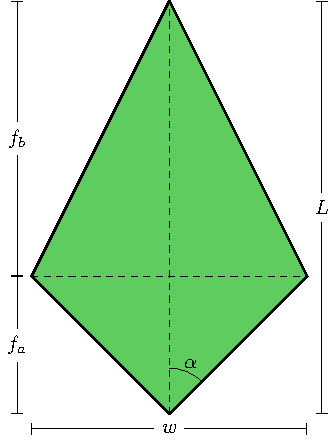
\includegraphics[width=3in]{frond}
	\captionof{figure}{Model frond diagram}
	\label{fig:frond}
\end{mcfig}

The frond is a kite with length $L$ from base to tip, and width $w$ from left to right.
 In figure \ref{fig:frond}, the base is shown at the bottom and the tip is shown at the top.
 The distance from the base to the diagonal connecting the left and right corners is called $f_a$, and the distance from that diagonal to the tip is called $f_b$.
 Clearly,
 \begin{equation}
	 f_a + f_b = L
 \end{equation}
 It is more convent to specify ratios than absolute lengths when considering a whole population with varying sizes.
 Let the following ratios be defined.
\begin{align}
	f_r &= \frac{L}{w} \\
	f_s &= \frac{f_a}{f_b}
\end{align}
These ratios are assumed to be consistent among the entire population, making them geometrically similar.
With these definitions, the shape of the frond can be fully specified by $L$, $f_r$, and $f_s$.
It is possible, then, to redefine $w$, $f_a$ and $f_b$ as follows from the preceding formulas.

\begin{align}
	w &= \frac{L}{f_r} \\
	f_a &= \frac{Lf_s}{1+f_s} \\
	f_a &= \frac{f_s}{1+f_s}
\end{align}

The angle $\alpha$, half of the angle from the base corner to the left and right corners, will be important in our model calculations.
Using the above equations and basic trigonometry, it can be found that
\begin{equation}
	\alpha = \tan^{-1}\left(\frac{2f_rf_s}{1+f_s}\right)
\end{equation}

\subsection{Variables}
The variables used in this model are summarized in the following table. Those with a check mark in the third column are inputs to the model. Those without a check mark are derived from the model inputs.
\begin{mcfig}
	\centering
	\begin{tabular}{@{}llc@{}} \toprule
		symbol       & description                         & input \\ \midrule
		$L$          & Frond length                        & \\
		$w$          & Frond width                         & \\
		$f_a$        & Inner frond length                  & \\
		$f_b$        & Outer frond length                  & \\
		$\alpha$     & Frond shape angle                   & \\
		$\theta_f$   & Frond direction angle               & \\
		$f_s$        & Frond shape parameter               & \checkmark \\
		$f_r$        & Frond length-width ratio            & \checkmark \\
		$v_w$        & Water current speed                 & \checkmark \\
		$\theta_w$   & Water current angle                 & \checkmark \\
		$\mu_L$      & Population mean frond length        & \checkmark \\
		$\sigma_L$   & Population frond length std. dev.   & \checkmark \\ \bottomrule
	\end{tabular}
	\captionof{figure}{Model variables}
	\label{fig:variables}
\end{mcfig}

\subsection{Population distributions}
As previously mentioned, the single frond which we are modeling is representative of a population.
While $f_r$ and $f_s$ are held constant among the entire population, $L$ and $\theta_f$ are assumed to vary according to the following distributions.

\subsubsection{Length distribution}

\begin{mcfig}
	\centering
	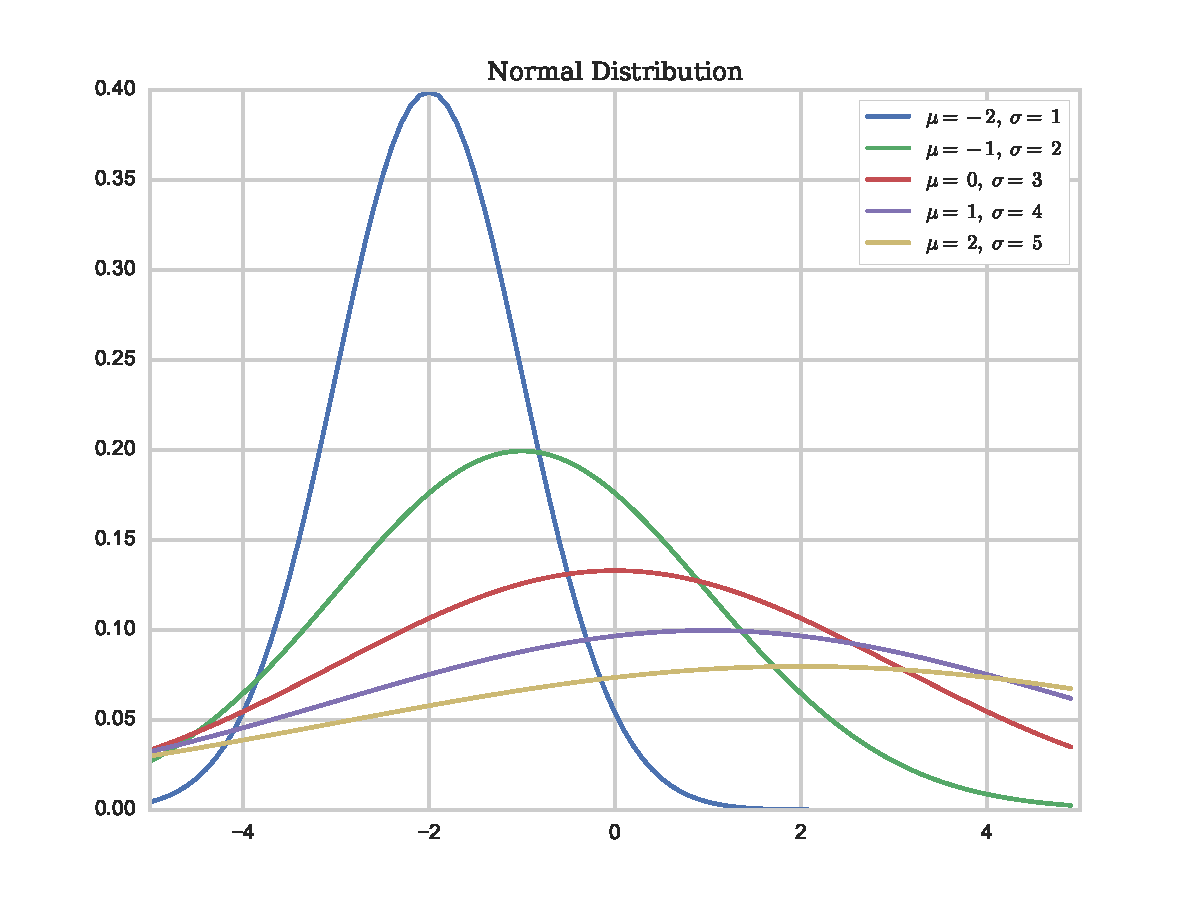
\includegraphics[width=\linewidth]{normal}
	\captionof{figure}{Normal distribution for a variety of parameters}
	\label{fig:normal}
\end{mcfig}

The frond length varies according to a normal distribution with mean $\mu_L$ and standard deviation $\sigma_L$. The probability density function (PDF) of this distribution is
\begin{equation}
	P_L(L) = \frac{1}{\sqrt{2\pi}\sigma_L} e^{-\frac{1}{2}\left(\frac{L-\mu_L}{\sigma_L}\right)^2}
\end{equation}

Notice that for a normal distribution,
\begin{equation}
	\displaystyle \lim_{\sigma \to \infty}P(x) = 0 \;\forall x \in \mathbb{R}
\end{equation}

The cumulative density function (CDF) is
\begin{equation}
	C_L(L) = \int_0^L P_L(\xi)\,d\xi = \frac{1}{2}\left(1-\erf\left(\frac{L-\mu_L}{\sqrt{2}\sigma_L}\right)\right)
\end{equation}

where $\erf$ is a non-elementary function called the error function, defined as
\begin{equation}
	\erf(x) = \int_0^x e^{-t^2}\,dt
\end{equation}

\subsubsection{Frond angle distribution}

\begin{mcfig}
	\centering
	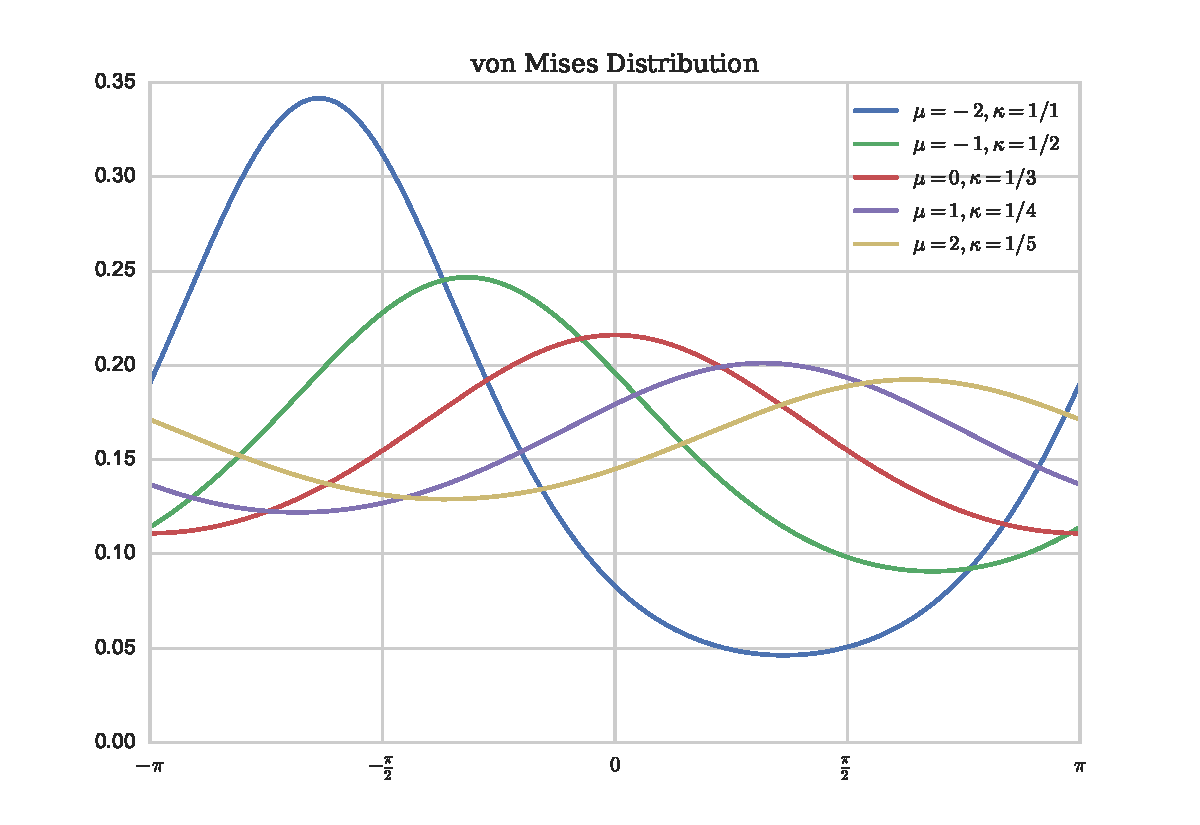
\includegraphics[width=\linewidth]{vonmises_2}
	\captionof{figure}{von Mises distribution for a variety of parameters}
	\label{fig:vonmises}
\end{mcfig}

The frond angle varies according to the von Mises distribution, which is the periodic analogue of the normal distribution.
It is defined on $[-\pi,\pi]$ rather than $(-\infty,\infty)$.
It has two parameters, $\mu$ and $\kappa$, which shift and sharpen the distribution respectively.
$\kappa$ can be considered analogous to $1/\sigma$ in the normal distribution.
Notice that unlike the normal distribution, the von Mises distribution approaches a \textit{non-zero} uniform distribution as $\kappa$ approaches 0.
\begin{equation}
	\displaystyle \lim_{\kappa \to 0}P(x) = \frac{1}{2\pi} \;\forall x \in [-\pi,\pi]
\end{equation}

The idea behind using this distribution is that without water current, the frond angles should be distributed uniformly, while as current velocity increases, they should be increasingly likely to be pointing in the direction of the current.
The way I have chosen to accomplish this is by using the von Mises distribution with $\mu = \theta_w$ and $\kappa = 1/v_w$.

The PDF for this distribution is
\begin{equation}
	P_{\theta_f}(\theta_f) = \frac{e^{(1/v_w)\cos(\theta_f-v_w)}}{2\pi I_0(1/v_w)}
\end{equation}
where $I_0(x)$ is the modified Bessel function of the first kind of order 0.

\subsubsection{Combined 2D length-angle distribution}
The previous two distributions are independent of one another. That is, the angle of the frond does not depend on the length, or vice versa.
Therefore, the probability of a frond simultaneously having a given frond length and angle is found as follows.

Given independent events $A$ and $B$,
\begin{equation}
	P(A \cap B) = P(A)P(B)
\end{equation}
Then the probability of frond length $L$ and frond angle $\theta_f$ coinciding is 
\begin{equation}
	P_{2D}(\theta_f,L) = P_{\theta_f}(\theta_f) \cdot P_L(L)
\end{equation}
A contour plot of this 2D distribution for a specific set of parameters is shown below, where probability is represented by color in the 2D plane. Darker green represents higher probability, while lighter beige represents lower probability.

\begin{mcfig}
	\centering
	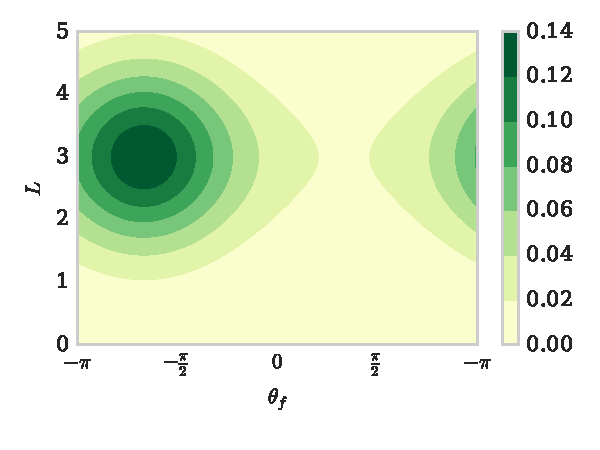
\includegraphics[width=\linewidth]{prob_2d}
	\captionof{figure}{2D length-angle probability distribution with \\$\mu_L=3,\sigma_L=1,\theta_f=2\pi/3,v_w=1$}
	\label{fig:dist_2d}
\end{mcfig}

\section{Model Analysis}
\subsection{Frond description}
\subsubsection{Relative coordinate system}
\label{sec:coords}
To determine under what conditions a frond will shade a given point, we begin by describing the shape of the frond in cartesian and then polar coordinates.
Of primary interest are the edges connected to the frond tip.
For convenience, we will use a relative coordinate system $(\theta',r)$ such that the line connecting the base to the tip is vertical, with the base at $(0,0)$.
The cartesian analogue of this coordinate system $(x',y')$ has the following properties.
\begin{align}
	x' &= r\cos\theta' \\ 
	y' &= r\sin\theta'
\end{align}
and
\begin{align}
	r &= \sqrt{x'^2+y'^2}
\end{align}
\vspace{-1em}
\begin{align}
	\theta' &= 
	\begin{cases}
		\tan^{-1}\left( \frac{y}{x} \right) & x > 0 \\
		\tan^{-1}\left( \frac{y}{x} \right) + \pi & x < 0 \\
		\frac{\pi}{2} & x = 0, y > 0 \\
		\frac{-\pi}{2} & x = 0, y < 0 \\
	\end{cases}
\end{align}

\subsubsection{Algebraic description}
With this coordinate system established, we can describe the outer two edges of the frond in cartesian coordinates as a piecewise linear function connecting the left corner: $(-w/2,f_a)$, the tip: $(0,L)$, and the right corner: $(w/2,f_a)$.
This function has the form
\begin{equation}
	y'_f(x') = L-\sign(x')\frac{f_b}{w/2}x'
\end{equation}
where
\begin{align}
	\sign(x) = 
	\begin{cases}
		1 & x > 0 \\
		0 & x = 0 \\
		-1 & x < 0 \\
	\end{cases}
\end{align}

Using the equations in section \ref{sec:coords}, this can be written in polar coordinates after some rearrangement as
\begin{equation}
	r_f(\theta') = \frac{L}{\sin\theta' + S(\theta')\frac{2f_b}{w}\cos\theta'}
\end{equation}
where
\begin{equation}
	S(\theta') = \sign(\theta'-\pi/2)
\end{equation}

Then, using the relationships in section \ref{sec:shape}, we can rewrite the above equation in terms of our model inputs.
\begin{equation}
	\label{eq:rf_rel}
	r_f(\theta') = \frac{L}{\sin\theta' + S(\theta')\frac{2f_r}{1+f_s}\cos\theta'}
\end{equation}

\subsubsection{Absolute Coordinates}
To generalize to a frond pointed at an angle $\theta_f$, we will use the coordinate system $(\theta,r)$ such that
\begin{equation}
	\theta = \theta' + \theta_f - \frac{\pi}{2}
\end{equation}

Then in terms of $\theta$, equation \ref{eq:rf_rel} becomes
\begin{equation}
	\label{eq:rf_abs}
	r_f(\theta - \theta_f + \frac{\pi}{2}) = \frac{L}{\sin\theta - \theta_f + \frac{\pi}{2} + S(\theta - \theta_f + \frac{\pi}{2})\frac{2f_r}{1+f_s}\cos\theta - \theta_f + \frac{\pi}{2}}
\end{equation}

\begin{mcfig}
	\centering
	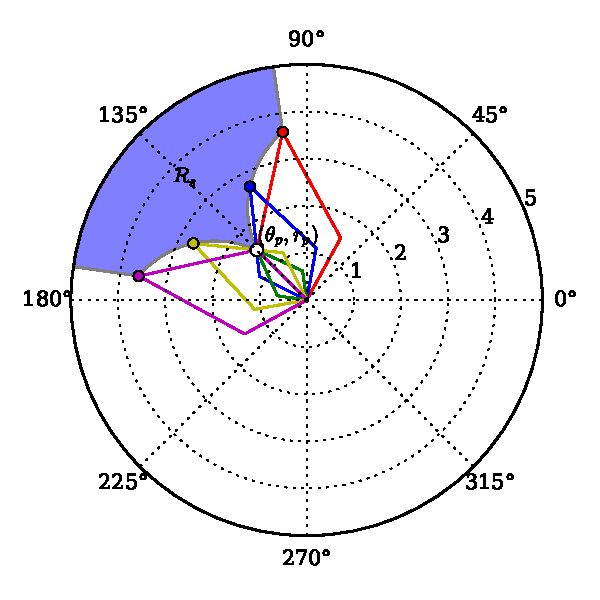
\includegraphics[width=\linewidth]{shade_area.pdf}
	\captionof{figure}{Outlines of minimum-length fronds for a variety of angles to shade the point $(\theta,r)=(3\pi/4,3/2)$}
	\label{fig:shade_area}
\end{mcfig}

\begin{mcfig}
	\centering
	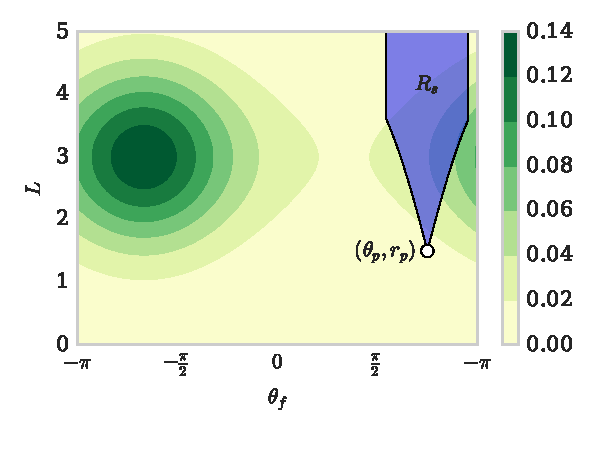
\includegraphics[width=\linewidth]{cart_shade}
	\captionof{figure}{Contour plot of $P_{2D}(\theta_f,L)$ overlayed with the region in the $\theta_f-L$ plane which results in shading of the point $(\theta,r)=(3\pi/4,3/2)$}
	\label{fig:cart_shade}
\end{mcfig}

\end{multicols}
\end{document}


